\chapter{MÉTHODOLOGIES ET MODÈLES}
\thispagestyle{empty}

\section{Conception conceptuelle}

\subsection{Vue d'ensemble de l'architecture système}

Le système de recommandation proposé suit une architecture en pipeline à trois couches (voir Figure~\ref{fig:system-architecture}) qui transforme séquentiellement les données brutes de Wikipédia en parcours d'apprentissage exploitables. Chaque couche est conçue pour être modulaire, permettant une expérimentation indépendante et une extension future.

\begin{figure}[H]
    \centering
    
\includegraphics[width=\textwidth]{figures/diagrams/architecture.png}
    \caption{Architecture système: pipeline à trois couches des données Wikipédia aux parcours d'apprentissage hiérarchiques.}
    \label{fig:system-architecture}
\end{figure}

\textbf{Couche 1 -- Préparation des Données:} La topologie du graphe WikiCS est chargée et enrichie avec le contenu textuel des articles récupéré via l'API Wikipédia. Le Wiki Stem Corpus fournit des données textuelles supplémentaires pour les articles. Le graphe résultant contient 11\,367 nœuds (articles CS) et 291\,039 arêtes dirigées (hyperliens).

\textbf{Couche 2 -- Embedding:} Deux processus d'embedding parallèles sont appliqués à chaque nœud. (a) \textit{Embedding Textuel}: les textes des articles sont encodés en utilisant BAAI/bge-m3 en vecteurs denses de 1024 dimensions capturant le contenu sémantique. (b) \textit{Node2Vec (basé sur SVD)}: une approche de factorisation de matrice PPMI produit des embeddings structurels de 128 dimensions reflétant le contexte de voisinage et la position de chaque nœud dans le graphe. Les deux vecteurs sont concaténés pour former un embedding combiné de 1\,152 dimensions par nœud, avec une pénalité de popularité normalisée par le degré appliquée à la composante structurelle.

\textbf{Couche 3 -- Recommandation et Présentation:} Étant donné une requête utilisateur, le système encode la requête avec le même modèle BGE-M3 et effectue une recherche de similarité dans l'espace d'embedding texte-structurel combiné. Les top-$k$ articles les plus similaires sont récupérés et passés à un LLM local pour générer un parcours d'apprentissage hiérarchique, qui est ensuite servi à l'utilisateur.

\subsection{Diagramme de flux de données}

La Figure~\ref{fig:data-flow} illustre le flux de données de bout en bout des données Wikipédia brutes à la sortie de recommandation finale. Le diagramme est structuré en deux pistes distinctes: une \textbf{piste hors ligne pré-calculée} (en haut) et une \textbf{piste en ligne au moment de la requête} (en bas).

\begin{figure}[H]
    \centering
    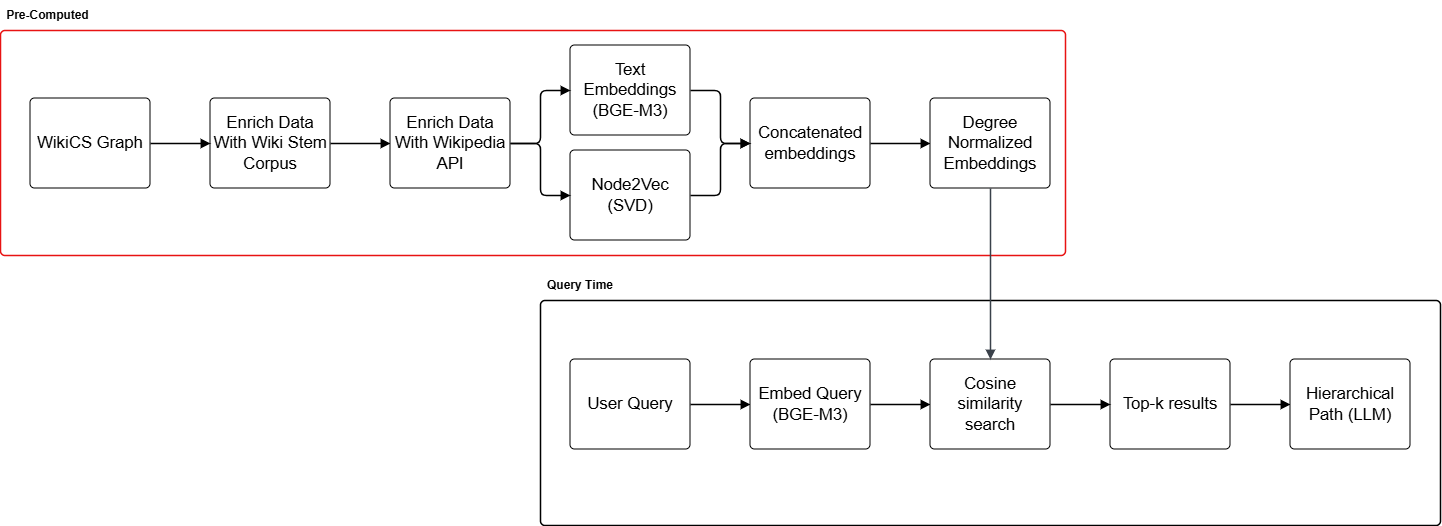
\includegraphics[width=\textwidth]{figures/diagrams/dataflow.png}
    \caption{Diagramme de flux de données: piste de pré-calcul hors ligne (en haut) et piste de recommandation au moment de la requête (en bas).}
    \label{fig:data-flow}
\end{figure}

\textbf{Piste Hors Ligne (Pré-Calculée):} Cette piste s'exécute une fois et met en cache tous les résultats pour les requêtes ultérieures.
\begin{enumerate}
    \item Le graphe WikiCS est chargé et enrichi avec les textes des articles du Wiki Stem Corpus et de l'API Wikipédia
    \item Les textes des articles sont encodés en parallèle via deux modèles: BAAI/bge-m3 (embeddings textuels 1024-dim) et Node2Vec basé sur SVD (embeddings structurels 128-dim)
    \item Les deux vecteurs d'embedding sont concaténés par nœud en une représentation combinée de 1\,152-dim
    \item Une pénalité de popularité normalisée par le degré est appliquée à la composante structurelle, produisant les embeddings finals mis en cache
\end{enumerate}

\textbf{Piste au Moment de la Requête:} Cette piste s'exécute en temps réel pour chaque requête utilisateur.
\begin{enumerate}
    \item L'utilisateur soumet une chaîne de requête de sujet
    \item La requête est encodée en utilisant le même modèle BAAI/bge-m3
    \item Le vecteur de requête est utilisé pour naviguer dans l'espace d'embedding texte-structurel combiné, identifiant les articles les plus sémantiquement pertinents
    \item Les top-$k$ candidats sont récupérés et classés par score de pertinence
    \item Les titres et métadonnées des articles sont passés à un LLM local, qui génère un parcours d'apprentissage hiérarchique et le retourne à l'utilisateur
\end{enumerate}

\subsection{Maquette d'interface}

La Figure~\ref{fig:mockup} présente une maquette de l'interface utilisateur attendue pour le système de recommandation.

\begin{figure}[H]
    \centering
    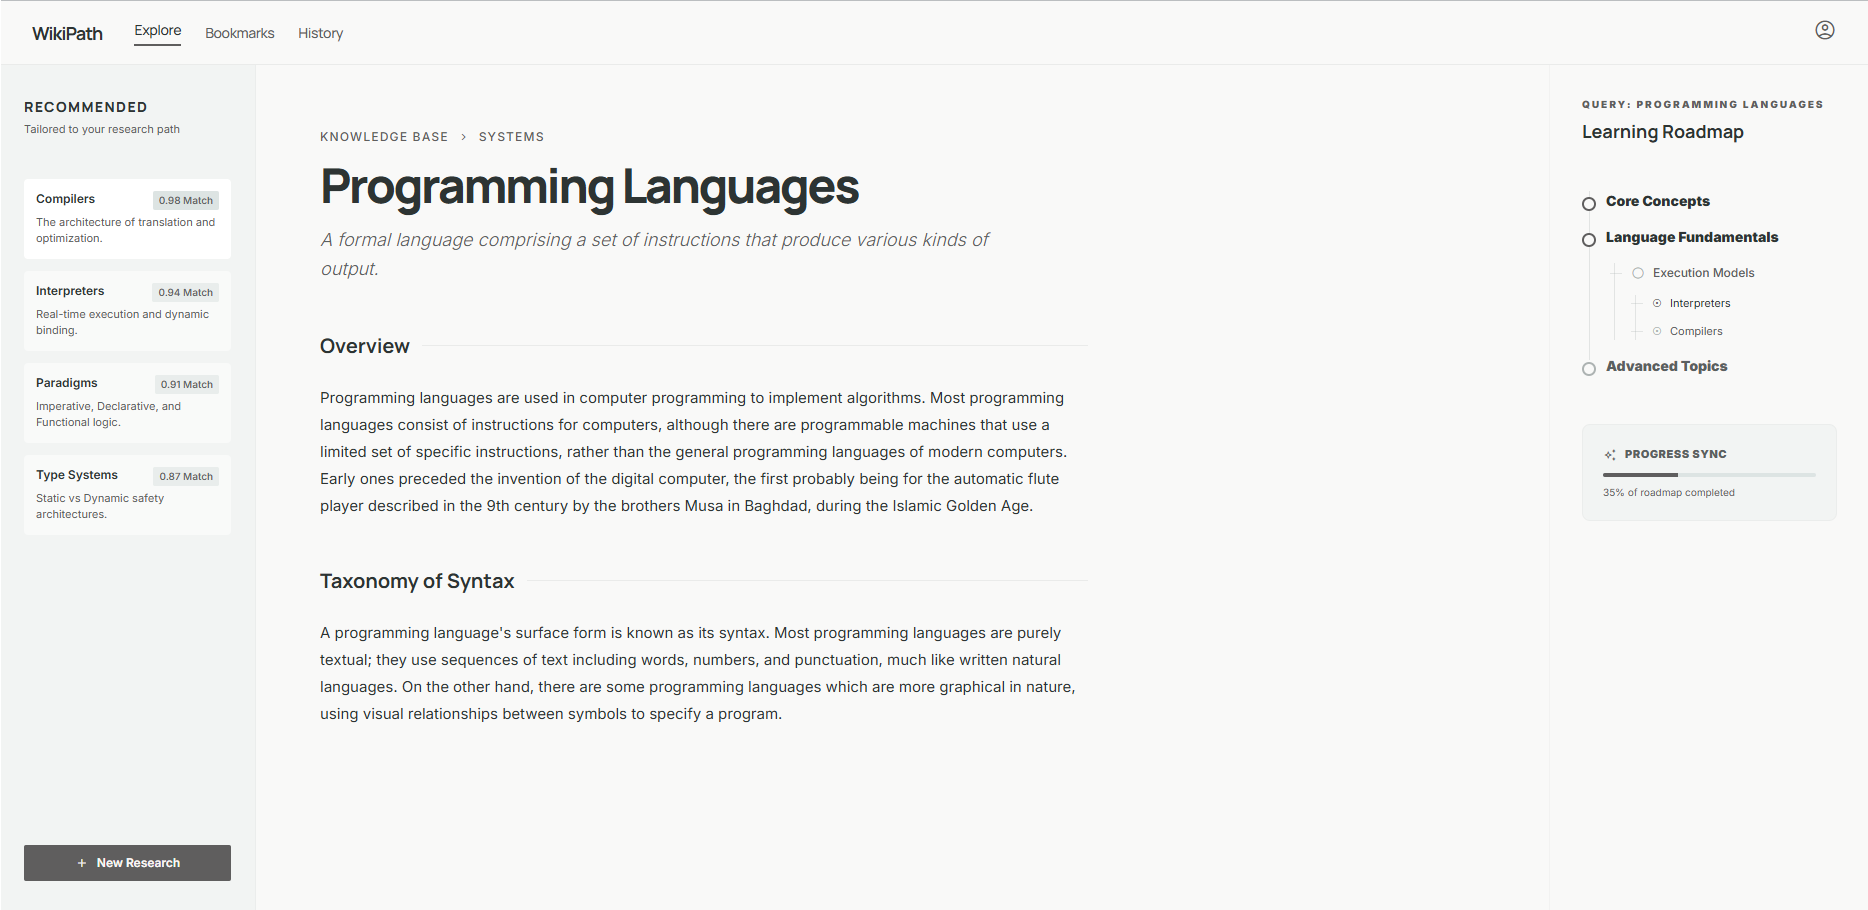
\includegraphics[width=\textwidth]{figures/diagrams/interface-mockup.png}
    \caption{Maquette haute-fidélité de l'interface de recommandation WikiPath.}
    \label{fig:mockup}
\end{figure}

L'interface suit une disposition à trois panneaux:
\begin{itemize}
    \item \textbf{Panneau gauche -- Articles Recommandés:} Affiche les top-$k$ articles récupérés avec leurs scores de similarité cosinus (ex. ``Compilers: 0.98 Match''). Chaque carte inclut le titre de l'article, une brève description et un indicateur de correspondance.
    \item \textbf{Panneau central -- Vue Article:} Affiche le contenu complet de l'article Wikipedia pour la recommandation actuellement sélectionnée, incluant le titre, le résumé et les sections.
    \item \textbf{Panneau droit -- Feuille de Route:} Présente le parcours d'apprentissage hiérarchique généré par LLM sous forme d'arbre pliable (ex. Core Concepts $\to$ Language Fundamentals $\to$ Execution Models $\to$ Interpreters / Compilers $\to$ Advanced Topics), accompagné d'un suivi de progression.
\end{itemize}

\subsection{Storyboard: Parcours utilisateur}

La Figure~\ref{fig:storyboard} illustre le parcours utilisateur en six étapes à travers le système de recommandation WikiPath.

\begin{figure}[H]
    \centering
    \includegraphics[width=\textwidth]{figures/diagrams/user-story.png}
    \caption{Storyboard du parcours utilisateur: de la saisie de la requête au parcours d'apprentissage hiérarchique.}
    \label{fig:storyboard}
\end{figure}

\begin{enumerate}
    \item \textbf{Saisie de la Requête:} L'utilisateur soumet une requête de sujet via l'interface de recherche (ex. ``Programming Languages'').
    \item \textbf{Encodage de la Requête:} La chaîne de requête est encodée en vecteur dense en utilisant BAAI/bge-m3, produisant une représentation de 1024 dimensions (ex. $[0.12, -0.74, \ldots]$).
    \item \textbf{Recherche de Similarité:} Le vecteur de requête encodé est utilisé pour naviguer dans l'espace d'embedding texte-structurel combiné, identifiant les articles les plus sémantiquement pertinents.
    \item \textbf{Classement des Candidats:} Les articles récupérés sont classés par score de similarité (ex. Compilers: 0.98, Interpreters: 0.94, Paradigms: 0.91, \ldots).
    \item \textbf{Structuration par LLM} \textit{[planifié]:} La liste plate classée est passée à un LLM local, qui organise les articles en une structure de prérequis hiérarchique.
    \item \textbf{Présentation du Parcours} \textit{[planifié]:} La hiérarchie organisée finale est affichée à l'utilisateur sous forme de carte conceptuelle (ex. Core Concepts $\to$ Language Fundamentals $\to$ Execution Models $\to$ Compilers / Interpreters).
\end{enumerate}

\section{Conception technique}

\subsection{Diagramme de composants UML}

La Figure~\ref{fig:component-diagram} présente le diagramme de composants UML montrant les principaux modules logiciels et leurs interactions.

\begin{figure}[H]
    \centering
    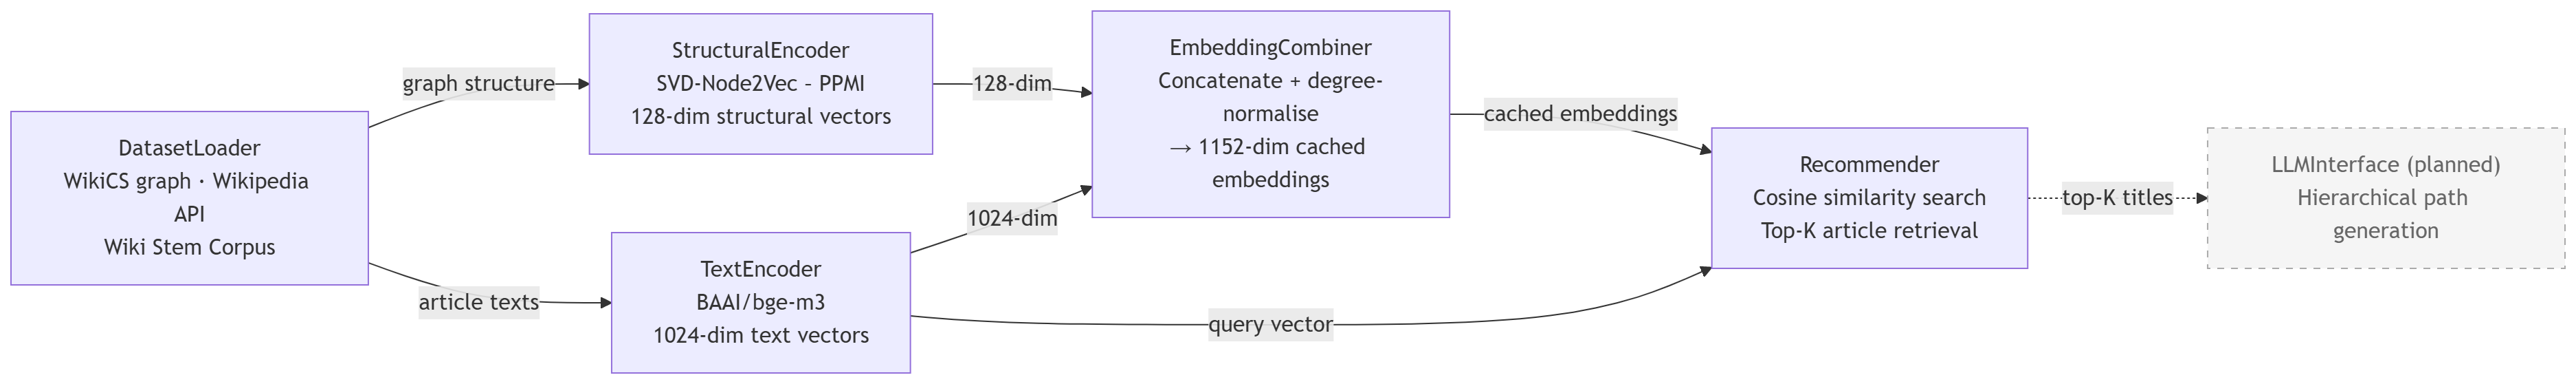
\includegraphics[width=\textwidth]{figures/diagrams/component-diagram.png}
    \caption{Diagramme de composants UML du système de recommandation WikiPath.}
    \label{fig:component-diagram}
\end{figure}

Le système est décomposé en six composants:

\begin{itemize}
    \item \texttt{DatasetLoader:} Charge la topologie du graphe WikiCS et l'enrichit avec les textes des articles récupérés de l'API Wikipédia et du Wiki Stem Corpus.
    \item \texttt{TextEncoder:} Enveloppe BAAI/bge-m3 pour encoder les textes des articles en vecteurs denses de 1024 dimensions. Également utilisé au moment de la requête pour encoder la requête utilisateur.
    \item \texttt{StructuralEncoder:} Implémente Node2Vec basé sur SVD via factorisation de matrice PPMI, produisant des embeddings structurels de 128 dimensions qui capturent le contexte de voisinage de chaque nœud.
    \item \texttt{EmbeddingCombiner:} Concatène les vecteurs textuels 1024-dim et structurels 128-dim en une représentation combinée de 1152-dim, applique une pénalité de popularité normalisée par le degré et met en cache le résultat sur disque.
    \item \texttt{Recommender:} Encode la requête utilisateur en utilisant \texttt{TextEncoder} et effectue une recherche de similarité guidée par le graphe dans l'espace d'embedding texte-structurel mis en cache pour récupérer les top-$k$ articles les plus pertinents. La stratégie de récupération exacte est sujette à raffinement en attente de l'approbation du superviseur.
    \item \texttt{LLMInterface} \textit{(planifié):} Enveloppera un LLM local servi via Ollama pour organiser la liste plate top-$k$ en parcours d'apprentissage hiérarchique. Pas encore implémenté.
\end{itemize}


\subsection{Mécanisme d'attention GAT}

Les Réseaux d'Attention sur Graphes (GAT)~\cite{velickovic2018graph} représentent une extension future planifiée du pipeline actuel. Alors que le système actuel utilise des embeddings combinés BGE-M3 et Node2Vec SVD pour les recommandations, le GAT sera étudié pour apprendre des représentations de nœuds enrichies en assistant sur le voisinage d'hyperliens. Le mécanisme d'attention procède comme suit:

\textbf{Étape 1 -- Transformation Linéaire:} Chaque nœud est transformé par une matrice de poids apprenable partagée $\mathbf{W} \in \mathbb{R}^{F' \times F}$:
\[
\vec{h}_i' = \mathbf{W} \vec{h}_i
\]

\textbf{Étape 2 -- Calcul du Coefficient d'Attention:} Le coefficient d'attention $e_{ij}$ entre les nœuds $i$ et $j$ est calculé comme:
\[
e_{ij} = \alpha(\mathbf{W}\vec{h}_i, \mathbf{W}\vec{h}_j) = \text{LeakyReLU}\!\left(\vec{a}^T \bigl[\mathbf{W}\vec{h}_i \, || \, \mathbf{W}\vec{h}_j \bigr]\right)
\]
où $\vec{a} \in \mathbb{R}^{2F'}$ est un vecteur d'attention apprenable et $||$ dénote la concaténation.

\textbf{Étape 3 -- Normalisation:} Les coefficients d'attention sont normalisés à travers tous les voisins en utilisant softmax:
\[
\alpha_{ij} = \text{softmax}_j(e_{ij}) = \frac{\exp(e_{ij})}{\sum_{k \in \mathcal{N}_i} \exp(e_{ik})}
\]

\textbf{Étape 4 -- Mise à Jour Multi-Tête:} Pour la stabilité et la capacité, $K$ têtes d'attention indépendantes sont utilisées en parallèle, et leurs sorties sont moyennées (ou concaténées):
\[
\vec{h}_i'' = \sigma\!\left(\frac{1}{K} \sum_{k=1}^K \sum_{j \in \mathcal{N}_i} \alpha_{ij}^k \mathbf{W}^k \vec{h}_j \right)
\]

\textbf{Couche GAT Complète:} La règle de propagation GAT complète est:
\[
\vec{h}_i^{(l+1)} = \sigma\!\left(\sum_{j \in \mathcal{N}_i} \alpha_{ij} \mathbf{W} \vec{h}_j^{(l)}\right)
\]

Pour une couche GAT à $K$ têtes, les sorties peuvent être concaténées:
\[
\vec{h}_i^{(l+1)} = \bigparallel_{k=1}^K \sigma\!\left(\sum_{j \in \mathcal{N}_i} \alpha_{ij}^k \mathbf{W}^k \vec{h}_j^{(l)}\right)
\]


\section{Méthodologie expérimentale}

\subsection{Dataset: Custom-WikiCS}

Le projet utilise le dataset Custom-WikiCS, une version modifiée du dataset benchmark Wiki-CS~\cite{mernyei2020wikics} évalué en utilisant les architectures GCN~\cite{kipf2017semi} et GAT~\cite{velickovic2018graph}:

\begin{itemize}
    \item \textbf{Nœuds:} 11\,367 articles CS Wikipedia (après suppression de 334 nœuds isolés)
    \item \textbf{Arêtes dirigées:} 291\,039 hyperliens
    \item \textbf{Arêtes non dirigées:} 216\,123 (chaque lien bidirectionnel compté une fois)
    \item \textbf{Features des nœuds:} Embeddings BAAI/bge-m3 de 1024 dimensions
    \item \textbf{Features supplémentaires:} Embeddings Node2Vec basés sur SVD de 128 dimensions
\end{itemize}

\subsection{Protocole d'évaluation}

La tâche de prédiction de liens suit le protocole d'évaluation standard:

\begin{itemize}
    \item \textbf{Arêtes positives:} Hyperliens existants dans le graphe
    \item \textbf{Arêtes négatives:} Paires de nœuds non connectés aléatoirement échantillonnées
    \item \textbf{Métriques:} ROC-AUC (Area Under the Receiver Operating Characteristic Curve)
    \item \textbf{Découpages:} Découpage 80\% train / 20\% test par nœud
\end{itemize}

Pour la tâche de recommandation:

\begin{itemize}
    \item \textbf{Métriques:} Hits@K (fraction des voisins de test dans le top-K) et MRR (Mean Reciprocal Rank)
    \item \textbf{Ligne de base:} Recommandation aléatoire (sélection d'article aléatoire)
\end{itemize}
